\subsection{O Método Osher}

O método Osher, baseado no limitador de variação total diminuída (TVD), é projetado para preservar a monotonicidade e minimizar oscilações em regiões com gradientes acentuados. Sua implementação utiliza fluxos numéricos controlados por um limitador, definido como:
\[
    \phi_{\text{lim}}(\theta) = \max(0, \min(1, \theta)),
\]
onde \(\theta\) é uma razão local dos gradientes calculados em cada ponto do domínio.

A solução numérica do método Osher é baseada na atualização iterativa da equação da advecção discretizada em um esquema de volumes finitos:
\[
    Q_i^{n+1} = Q_i^n - C (F_{i+1/2} - F_{i-1/2}),
\]
com o fluxo \(F_{i+1/2}\) controlado pelo limitador \(\phi_{\text{lim}}\).

\begin{figure}[H]
    \centering
    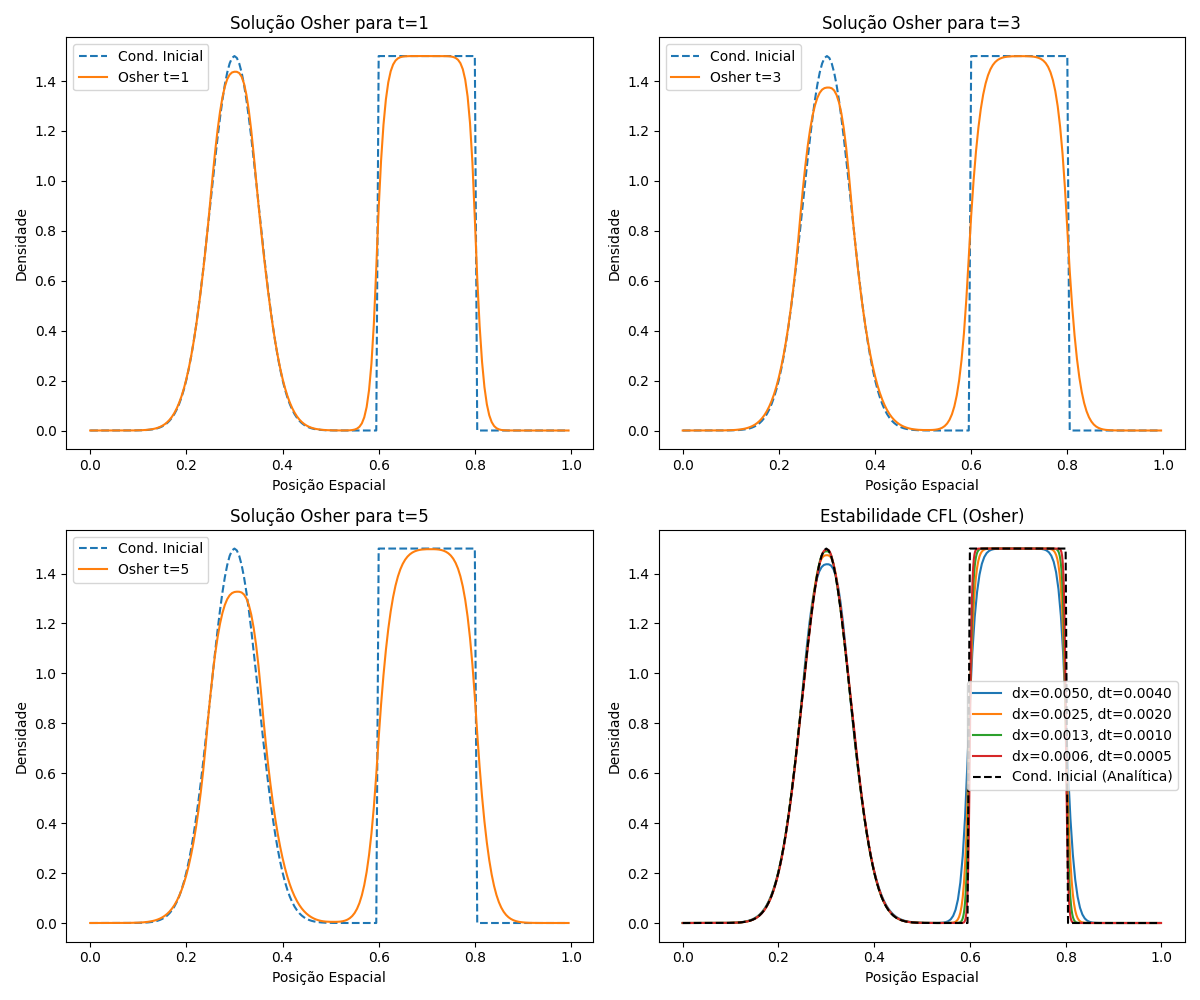
\includegraphics[width=\textwidth]{code/images/Osher.png}
    \caption{Solução Osher para $t=1$, $t=3$ e $t=5$, com a condição inicial representada pela linha tracejada.}
    \label{fig:osher}
\end{figure}

\subsection{Análise dos Resultados do Método Osher}

A Figura \ref{fig:osher} apresenta a evolução da solução obtida pelo método Osher nos tempos \(t=1\), \(t=3\) e \(t=5\), comparando a solução numérica com a condição inicial (\(t=0\)).

- \textbf{Condição inicial (\(t=0\))}: A condição inicial utilizada é uma combinação de uma função gaussiana centrada em \(x=0,3\) e uma concentração uniforme entre \(x=0,6\) e \(x=0,8\).
- \textbf{Incremento de tempo (\(\Delta t\))}: O número de Courant \(C=0,8\) foi aplicado para calcular o passo de tempo, garantindo estabilidade conforme a condição CFL.

Os gráficos mostram que o método Osher preserva de forma eficiente a monotonicidade e a forma geral do perfil de concentração ao longo do tempo, minimizando oscilações. Em \(t=1\), a solução numérica está bem próxima da condição inicial, com pequenas diferenças no topo da gaussiana e nas bordas da concentração uniforme. Para \(t=3\) e \(t=5\), o método continua apresentando um comportamento estável, preservando a forma da gaussiana e do degrau, mas com leves atenuações devido à dissipação numérica.

\begin{table}[H]
    \centering
    \begin{tabular}{rrrrrr}
\toprule
Posicao Espacial & Condicao Inicial & Osher t=1 & Osher t=3 & Osher t=5 & Posicao da Estabilidade \\
\midrule
0.000000 & 0.000000 & 0.000000 & 0.000002 & 0.000006 & 0.000000 \\
0.050000 & 0.000006 & 0.000012 & 0.000034 & 0.000053 & 0.050000 \\
0.100000 & 0.000503 & 0.000718 & 0.001223 & 0.001420 & 0.100000 \\
0.150000 & 0.016663 & 0.018961 & 0.023321 & 0.022593 & 0.150000 \\
0.200000 & 0.203003 & 0.206288 & 0.213317 & 0.192373 & 0.200000 \\
0.250000 & 0.909796 & 0.923582 & 0.967856 & 0.912867 & 0.250000 \\
0.300000 & 1.500000 & 1.437160 & 1.373804 & 1.325958 & 0.300000 \\
0.350000 & 0.909796 & 0.904268 & 0.930223 & 1.030586 & 0.350000 \\
0.400000 & 0.203003 & 0.208248 & 0.218056 & 0.261015 & 0.400000 \\
0.450000 & 0.016663 & 0.019849 & 0.025923 & 0.037466 & 0.450000 \\
0.500000 & 0.000503 & 0.000766 & 0.001917 & 0.004691 & 0.500000 \\
0.550000 & 0.000006 & 0.003678 & 0.028017 & 0.040087 & 0.550000 \\
0.600000 & 1.500000 & 0.890163 & 0.860449 & 0.740881 & 0.600000 \\
0.650000 & 1.500000 & 1.497814 & 1.475949 & 1.438465 & 0.650000 \\
0.700000 & 1.500000 & 1.500000 & 1.499627 & 1.497384 & 0.700000 \\
0.750000 & 1.500000 & 1.498258 & 1.481938 & 1.472013 & 0.750000 \\
0.800000 & 1.500000 & 0.849292 & 0.804179 & 0.905699 & 0.800000 \\
0.850000 & 0.000000 & 0.004615 & 0.036054 & 0.083578 & 0.850000 \\
0.900000 & 0.000000 & 0.000001 & 0.000308 & 0.002432 & 0.900000 \\
0.950000 & 0.000000 & 0.000000 & 0.000003 & 0.000025 & 0.950000 \\
\bottomrule
\end{tabular}

    \caption{Resultados numéricos do método Osher para posições espaciais selecionadas em $t=1$, $t=3$ e $t=5$.}
    \label{tab:osher}
\end{table}

A Tabela \ref{tab:osher} apresenta os valores numéricos da solução do método Osher em posições selecionadas do domínio para diferentes instantes de tempo. Os resultados evidenciam a precisão do método em capturar a evolução do perfil de concentração com o mínimo de oscilações ou dispersão.

\subsection{Implementação em Python}

O código em Python para o método Osher utiliza a função principal \texttt{resolverAdveccaoTVD}, que aplica o limitador e calcula a evolução da densidade ao longo do tempo. A cada passo temporal, o fluxo \(F_{i+1/2}\) é atualizado com base no limitador de Osher, garantindo estabilidade e precisão. O trecho do código é apresentado na Listagem~\ref{lst:codigo_osher}.

\begin{lstlisting}[language=Python, caption={Código para resolver a advecção usando o método Osher}, label={lst:codigo_osher}]
# Método TVD com limitador de Osher
def limitadorOsher(theta):
    return np.maximum(0, np.minimum(1, theta))

def metodoTvdOsher(densidade, nt, intervaloTempo, intervaloEspacial, numeroCourant):
    """
    Método TVD para resolver a advecção utilizando o limitador de Osher.
    """
    for n in range(nt):
        novaDensidade = densidade.copy()
        for i in range(len(densidade)):
            esquerda = (i - 1) % len(densidade)
            direita = (i + 1) % len(densidade)
            # Calcula o gradiente relativo (theta)
            theta = (densidade[i] - densidade[esquerda]) / (densidade[direita] - densidade[i] + 1e-6)
            # Fluxos para direita e esquerda
            fluxoDireita = densidade[i] + 0.5 * numeroCourant * (1 - numeroCourant) * limitadorOsher(theta) * (densidade[direita] - densidade[i])
            fluxoEsquerda = densidade[esquerda] + 0.5 * numeroCourant * (1 - numeroCourant) * limitadorOsher(theta) * (densidade[i] - densidade[esquerda])
            # Atualiza a densidade
            novaDensidade[i] = densidade[i] - numeroCourant * (fluxoDireita - fluxoEsquerda)
        densidade = novaDensidade.copy()
    return densidade
\end{lstlisting}


A implementação do método Osher utiliza o limitador \texttt{limitadorOsher} para controlar os fluxos numéricos em cada passo temporal, garantindo estabilidade e precisão. O número de Courant \(C = 0,8\) é aplicado para satisfazer a condição CFL, essencial para a convergência das soluções numéricas.
